
\chapter {Две жизни}

\begin{remark}
Как прожить две жизни. Одну — крутым диверсантом. Вторую — эффективным менеджером.
\end{remark}


Чувак в 49 лет захотел руководить стартапом. Публично пообещал, что заработает миллионы. На сельском хозяйстве. Будучи инвалидом.
В воюющей стране. При социализме. При Сталине.
(пост для тех, кто жалуется на плохие стартовые условия)

Имя: Кирилл Прокофьевич Орловский
Возраст: 49 лет.
Здоровье: Правая рука ампутирована по плечо. На левой руке остался один палец. Слух повреждён на 50%.
\begin{figure}[h!tb] 
	\centering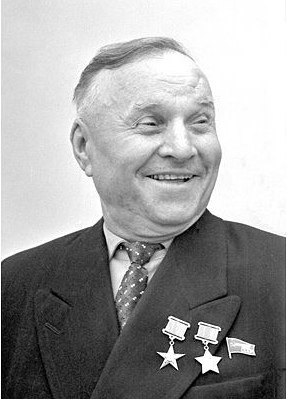
\includegraphics[scale=0.4]{Orlovskiy/TLiUJ3qpZuA.jpg}
	%	\label{fig:scipion} % Unique label used for referencing the figure in-text\end{document}
	%	%\addcontentsline{toc}{figure}{Figure \ref{fig:placeholder}} % Uncomment to add the figure to the table of contents%----------------------------------------------------------------------------------------
	\caption{Орловский}%	CHAPTER 2
\end{figure}
Опыт и навыки: 29 лет службы в разведке. Профессиональный диверсант и организатор партизанских отрядов. Начал партизанить в Белоруссии ещё в Первую мировую. Успел повоевать в Испании (снова в тылу врага) — попал в прототипы книги Хемингуэя.

Хватило бы на сериал с эффектной концовкой. Концовка — 1943 год, белорусские леса. По зимней дороге едет секретная колонна, с группой высших офицеров. Едут на охоту на кабанов. По данным разведки — с ними же едет Вильгельм Кубе, гауляйтер всей Белоруссии.

А в группе партизан всего 12 человек, маловато для хорошей засады. Времени, чтобы собрать отряд побольше, не было. Птичка могла ускользнуть, Орловский решил рискнуть.

Залегли в снег в маскхалатах, пропустили колонну. Решили атаковать их на обратном пути, когда вечером поедут с охоты. 12 часов ждали в снегу, не шевелясь. И вот скоротечный бой. Немцев положили всех, забрали трофеи и документы (гауляйтера среди фрицев не оказалось). Наши без потерь — только один тяжело раненый и контуженный, командир. Неудачно бросил взрывчатку. Довоевался.

Орловского лечили в отряде. Гангрена, ампутация в полевых условиях. Летом эвакуировали в Москву. Вручили звезду Героя Советского Союза. Обеспечили квартирой и пенсией, сказали «отдыхай, ты своё отвоевал». Это была его вторая отставка (в 1938 уже отправляли на пенсию по состоянию здоровья, но потом вызвали обратно на войну).

Вот и конец сериала. Последняя сцена — гауляйтера Кубе всё-таки достали партизаны. Ребята из минского подполья заминировали кровать в его особняке. Взлетел на воздух в сентябре 43-го.

Прошёл год. Что делает наш герой? Просится на фронт? (прецеденты есть, воевали и без обеих рук). Нет, понимает, что в бою может и не выдержать. Пишет мемуары? Тоже нет.

Он пишет БИЗНЕС-ПЛАН.

Оказывается, все эти годы у Орловского было хобби, которое он теперь захотел превратить в профессию.

Все эти годы в тылу врага, в перерывах между диверсиями он выписывал и читал журналы по сельскому хозяйству.
А когда в 39-40 гг работал на гражданке (проректором в сельхоз вузе) — успел там же поучиться студентом.

Не говоря о том, что в юности исходил пешком всю Белоруссию. Знал каждую кочку в каждой деревне. Нахватался знаний.

И вот Орловский задумал взять под управление колхоз в родной деревне и за пять лет превратить его в прибыльное предприятие. Расчертил по карте схему полей. Рассчитал постройки и лесополосы. Написал подробную смету.
Цель — выручка 3 миллиона рублей в год к 1950 году.
(в довоенном 1940 году колхоз произвел продукции на 167 тысяч)
\begin{figure}[h!tb] 
	\centering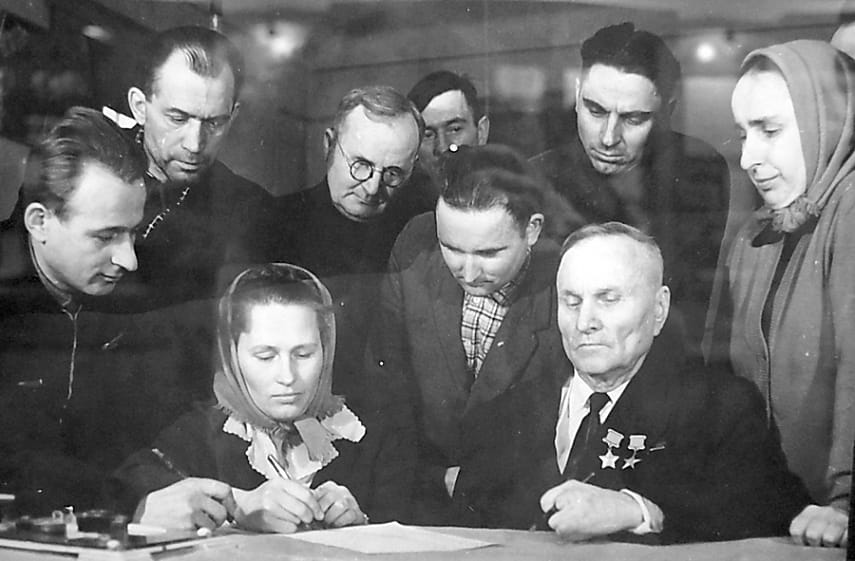
\includegraphics[scale=0.4]{Orlovskiy/Af8WSw9knQM.jpg}
	%	\label{fig:scipion} % Unique label used for referencing the figure in-text\end{document}
	%	%\addcontentsline{toc}{figure}{Figure \ref{fig:placeholder}} % Uncomment to add the figure to the table of contents%----------------------------------------------------------------------------------------
	\caption{Уже в колхозе}%	CHAPTER 2
\end{figure}
А на дворе 44-год, Белоруссия ещё под немцем!
Освободим мы скоро территорию, а где средства брать на эти наполеоновские планы? Семена, стройматериалы, технику?

В бизнес-плане всё учтено.
Естественно, нужны средства.

Инвестор должен выделить 125 тысяч рублей деньгами, и 2,175 миллиона — семенами, материалами, техникой.
Взамен инвестор получает долю 100%.

Риски инвестора — да почти никаких. Неуспешных и убыточных колхозов пруд пруди. Одним больше, какая разница?

Риски Орловского — известное дело, арест. Не посмотрели бы, что герой.

Сам ввязался, понимает, на что идёт.

В итоге, 6 июля 1944 года он направляет письмо главному бизнес-ангелу и лучшему другу колхозников, Сталину.
Почитайте письмо, это отдельный пример, как писать просто и убедительно.

Сначала факты из биографии и бизнес-план. А посередине абзац с мотивацией, трогает за душу:
«...материально я живу очень хорошо. Морально — плохо...»

(письмо целиком: \url{https://www.sb.by/articles/i-gitler-khotel-pobedit-takikh-lyudey.html})

Сталин одобрил затею и выдал кредит.
В январе 1945 Орловский становится председателем колхоза «Рассвет» в родной деревне Мышковичи.

А дальше — долгая изнурительная работа.

Снизу — всё плохо. Обезлюдевшая деревня, мужиков нет. Подрастающая молодёжь стремится любой ценой уехать из колхоза, чтобы вырваться из нищеты.
\begin{figure}[h!tb] 
	\centering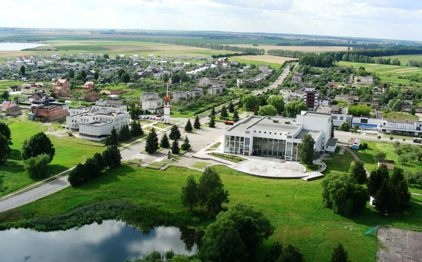
\includegraphics[scale=0.6]{Orlovskiy/3OfP7SDYNgM.jpg}
	%	\label{fig:scipion} % Unique label used for referencing the figure in-text\end{document}
	%	%\addcontentsline{toc}{figure}{Figure \ref{fig:placeholder}} % Uncomment to add the figure to the table of contents%----------------------------------------------------------------------------------------
	\caption{Как это все выглядит сейчас}%	CHAPTER 2
\end{figure}
Сверху свои заморочки. Твоё начальство — район, а над ними сверху обком. Всем нужен план по заготовкам, а лучше перевыполнение плана.

Колхозникам за работу ставят палочки (отмечают в табеле трудодни). Подразумевается, что доля от собранного урожая пойдёт им в счёт оплаты.
\begin{figure}[h!tb] 
	\centering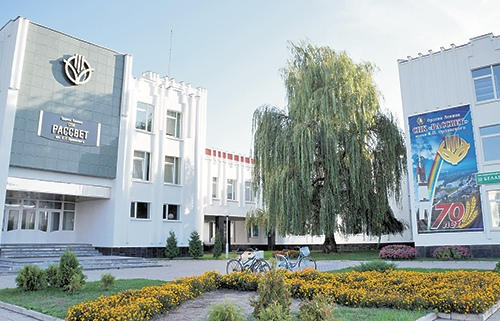
\includegraphics[scale=0.6]{Orlovskiy/91GAr5Oq6nA.jpg}
	%	\label{fig:scipion} % Unique label used for referencing the figure in-text\end{document}
	%	%\addcontentsline{toc}{figure}{Figure \ref{fig:placeholder}} % Uncomment to add the figure to the table of contents%----------------------------------------------------------------------------------------
	\caption{Как это все выглядит сейчас. Еще фото}%	CHAPTER 2
\end{figure}
Как хороший руководитель, ты откладываешь часть зерна, чтобы осенью заплатить колхозникам, сдержать обещание.

А в районе говорят — зерна собрано мало, нужно сдать всё, колхозники как-нибудь проживут и так. Зерно забрали, платить колхозникам нечем. Как смотреть людям в глаза?

Техника. Своей техники в колхозе нет. Вся техника района сосредоточена на МТС. Те выезжают на колхозные поля по очереди. Выбил технику по своей заявке — молодец. Не выбил — твои женщины пашут на коровах, а убирают серпами.

Вот и крутись. Будь тем человеком, кому больше всех надо. Умудряйся угодить всем. Работников — удержать, заставить работать. Начальству — угодить или схитрить, обмануть. При этом не забывать о стратегии — засеивать поля, сажать лесополосы и сады, строить фермы и жильё.

И где-то там ждёт возврата своих инвестиций инвестор. Успеешь к 50-му году?

Успел. Колхоз «Рассвет» стал первым послевоенным колхозом-миллионером. Не Кубань или Ставрополье вырвались в лидеры — Белоруссия! (факт не проверял, так написано в википедии).

В 1958 году Орловский получил героя соцтруда — вторая звезда на груди.

В 1965 на экраны выходит фильм «Председатель» с Михаилом Ульяновым — по мотивам биографии Кирилла Орловского. Фильм очень сильный, посмотрите, не пожалеете.

Орловский работал председателем до самой смерти в 1968 году.
Оставил после себя успешный колхоз и богатую деревню.

Вот такая жизнь, дай бог каждому.

Выводы для начинающих предпринимателей:
\begin{enumerate}
	\item  Возраст не помеха.
\item  Нет рук — не проблема, главное, что есть голова.
\item  Прошлый опыт и навыки — очень важно, это ваш главный актив.
\item  Если вам 45 и вы уже на пенсии — не стесняйтесь торчать на лекциях вместе со студентами, если вам нравится предмет.
\item  Когда пишете бизнес-план — постарайтесь. Представьте, что будете его презентовать Сталину.
\item  Считайте, что отвечаете за успех своей жизнью. Когда выбили инвестиции — идите до конца.
\end{enumerate}

\begin{figure}[h!tb] 
	\centering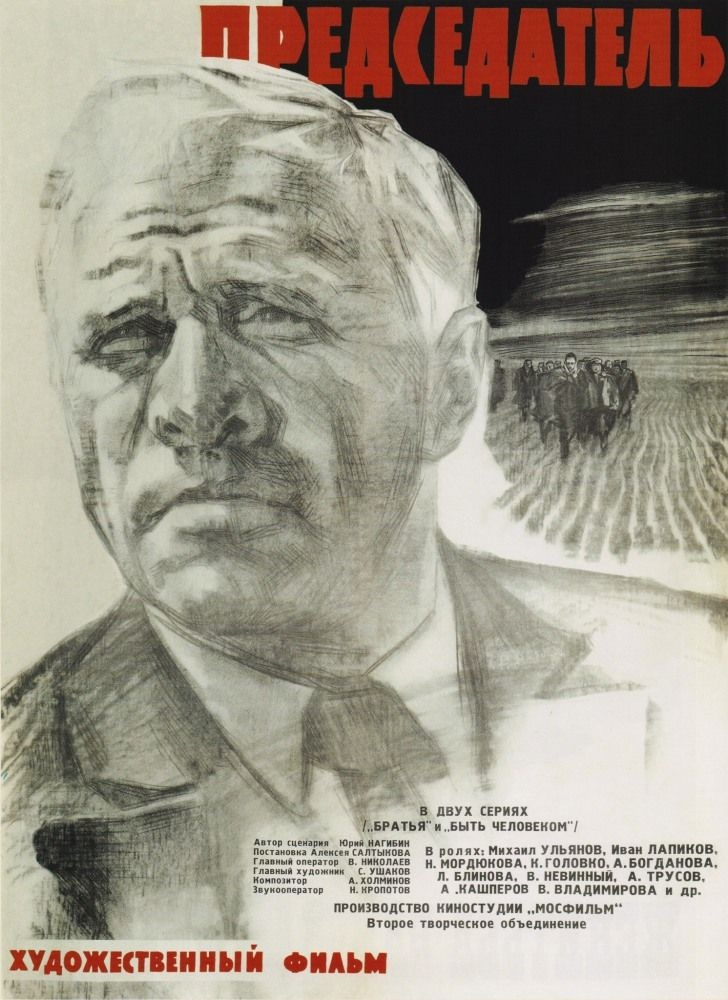
\includegraphics[scale=0.4]{Orlovskiy/CdCLdInaVq8.jpg}
	%	\label{fig:scipion} % Unique label used for referencing the figure in-text\end{document}
	%	%\addcontentsline{toc}{figure}{Figure \ref{fig:placeholder}} % Uncomment to add the figure to the table of contents%----------------------------------------------------------------------------------------
	\caption{Фильм об этом всем}%	CHAPTER 2
\end{figure}


Автор Юрий Деточкин.  Оригинал \url{https://vk.com/wall-162479647_139584}

\#Деточкин@catx2
\#Заметка@catx2

